\documentclass[journal, onecolumn]{IEEEtran}

\usepackage{biblatex}


\usepackage[fleqn]{amsmath}
\usepackage{amssymb}
\usepackage{graphicx}
\usepackage{cancel}
\usepackage{tabularx}
\usepackage{algorithm}
\usepackage{algorithmic}
\usepackage{parskip}
\usepackage{graphicx,wrapfig,lipsum}

\usepackage{bookmark}

% \usepackage{caption}
% \usepackage{subcaption}

\usepackage{subfig}
% \usepackage[authordate,autocite=inline,backend=biber,sorting=nyt,natbib=true]{biblatex}
% \addbibresource{citations.bib}


\usepackage{harpoon}
% \newcommand*{\vect}[1]{\overrightharp{\ensuremath{#1}}}

\newcommand{\vect}{\overset{\rightharpoonup}}
\newcommand{\bvect}[3]{\begin{bmatrix}
    #1 \\
    #2 \\
    #3
\end{bmatrix}}
\newcommand{\bvecttrans}[3]{\begin{bmatrix}
    #1 & #2 & #3
\end{bmatrix}^{T}}
\newcommand{\bvectdot}[3]{\begin{bmatrix}
    \dot{#1} \\
    \dot{#2} \\
    \dot{#3}
\end{bmatrix}}

\newcommand\norm[1]{\lVert#1\rVert}

\graphicspath {{images}}

\usepackage{hyperref}
\hypersetup{
colorlinks=false,
linkcolor=blue,
filecolor=magenta,
    urlcolor=blue,
}
\urlstyle{same}

\begin{document}

\title{Quadcopter Differential Equations of Motion}
\author{Jonathan~Dorsey  \\  \url{https://github.com/JonnyD1117/}}

% \IEEEmembership{Member: No Sleep Club: est. 2017}
\markboth{Journal of Graduate School Assignments March~2023}

\maketitle

\section{Introduction}

These are my notes on the derivations and formulation for the 6-DOF Quadcopter rigid body dynamics equations of motion, making notes on all salient aspects concerning details from derivation to implementation in C++.


\section{Coordinate Systems and Frames of Reference}

\subsection{Inertial Frame of Reference}
The inertial reference frame is defined as a coordinate system that is not accelerating or rotating. Typically, the earth is chosen to be the inertial reference frame of the vehicle.


\subsection{Euler Angles}

Euler Angles are a series of sequential rotations for a given coordinate system. This formulation is commonly used to convert between different coordinate systems. \newline

The most common symbols for \textbf{Euler Angles} in aircraft dynamics are $\theta$ (pitch), $\psi$(yaw), $\phi$(rolls)

 \begin{figure}[h]
    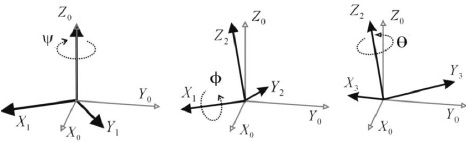
\includegraphics[width=10cm]{euler_frames}
    \centering
    \label{fig:euler_angles}
    \caption{Sequential Rotations of Euler Angles}
\end{figure}

\subsubsection{Euler Rotation Matrix}

By using trigonometry, between each pair of coordinates above it is possible to show that rotations between frames can be expressed as the product of elementary rotation matrices obtained from each rotation about intermediate axes. 

$$
R_{x}(\phi) = \begin{bmatrix}
    1 & 0 & 0\\ 
    0 & c(\phi) & -s(\phi)\\
    0 & s(\phi) & c(\phi)
\end{bmatrix} \quad
R_{y}(\theta) = \begin{bmatrix}
    c(\theta) & 0 & s(\theta)\\
    0 & 1 & 0\\
    -s(\theta) & 0 & \c(\theta)
\end{bmatrix} \quad
R_{z}(\psi) = \begin{bmatrix}
    c(\psi) & -s(\psi) & 0\\
    s(\psi) & c(\psi) & 0\\
    0 & 0 & 1
\end{bmatrix}  $$ 

These elementary rotation matrices can be combined to to produce a single rotation matrix. 

$$ R_{zyx}(\phi, \theta, \psi)\biggr\rvert_{B}^{I} = R_{x}(\phi) \cdot R_{y}(\theta) \cdot R_{z}(\psi)$$

$$ R_{zyx}(\phi, \theta, \psi)\biggr\rvert_{B}^{I} = \begin{bmatrix}
    c(\theta)c(\psi) & s(\phi)s(\theta)c(\psi)-c(\phi)s(\psi) & c(\phi)s(\theta)c(\psi)+s(\theta)s(\psi)\\
    c(\theta)s(\psi) & s(\phi)s(\theta)s(\psi)+c(\phi)c(\psi) & c(\phi)s(\theta)s(\psi)-s(\theta)c(\psi)\\
    -s(\theta) & s(\phi)c(\theta) & c(\phi)c(\theta)
\end{bmatrix}$$

It should also be noted that since this rotation matrix is orthogonal, it's inverse can be found by taking the transpose... 

$$ R^{-1} = R^{T}$$

\subsubsection{Euler Rates to Angular Velocity Components (\& Vise Versa)}

$$ T(\phi, \theta, \psi) = \begin{bmatrix}
    1 & s(\phi)t(\theta) & c(\phi)t(\theta)\\
    0 & c(\phi) & -s(\phi)\\
    0 & \frac{s(\phi)}{c(\theta)} & \frac{c(\phi)}{c(\theta)}
\end{bmatrix}$$



$$\bvectdot{x}{y}{x} = R(\phi, \theta, \psi) \cdot \bvect{u}{v}{w} \quad , \quad  \bvectdot{\phi}{\theta}{\psi} = T(\phi, \theta, \psi) \cdot \bvect{p}{q}{r} $$

It should be noted that the body frame angular velocities are not equal to the Euler rates. This is due to the fact that the angular velocity components exist simultaneously as components of the angular velocity vector $\vect{\omega}$. However, Euler angles do not exist at the same time, they constitute a sequence of three consecutive rotations around different axes of rotations. 



$$\bvectdot{p}{q}{r} = \bvect{\dot{\phi}}{0}{0} + R() \bvect{0}{\dot{\theta}}{0} + R()R() \bvect{0}{0}{\dot{\psi}}$$

These transformations convert between the angular velocity and the euler rates (and vise versa)

$$ \bvect{p}{q}{r} = \begin{bmatrix}
    1 & 0 & -s(\theta)\\
    0 & c(\phi) & s(\phi)c(\theta)\\
    0 & -s(\phi) & c(\phi)c(\theta) \end{bmatrix}  \bvectdot{\phi}{\theta}{\psi}$$

$$ \bvectdot{\phi}{\theta}{\psi} = \begin{bmatrix}
    1 & s(\phi)t(\theta) & c(\phi)t(\theta)\\
    0 & c(\phi) & -s(\phi)\\
    0 & \frac{s(\phi)}{c(\theta)} & \frac{c(\phi)}{c(\theta)} \end{bmatrix} \bvect{p}{q}{r} $$

\subsubsection{Problem with Euler Angles}
The main drawback of using Euler angles is the presence of gimbal lock where there does not exist a unique mathematical description of the orientation given the angles. 

\subsection{Quaternions}
The most commonly used alternative to Euler angles is the quaternion formulation. 

$$ 
q = q_{0} + q_{1}\hat{i} + q_{2}\hat{j} + q_{3}\hat{k} 
$$
$$q = \begin{bmatrix}
    q_0  & q_1 &  q_2 & q_3
\end{bmatrix}^{T}$$

\subsubsection{Quaternion Properties}

The product of two quaternions is defined as the Kronecker product as defined below.

$$p \times q = \begin{bmatrix}
    p_0q_0 - p_1q_1 - p_2q_2 - p_3q_3 \\
    p_0q_1 + p_1q_0 + p_2q_3 - p_3q_2 \\
    p_0q_2 - p_1q_3 + p_2q_0 + p_3q_1 \\
    p_0q_3 + p_1q_2 - p_2q_1 + p_3q_0
\end{bmatrix}$$


A quaternion can be represented as a $4x4$ matrix given $q = [q_0, q_1, q_2, q_3]$... 

$$\begin{bmatrix}
    q_0 & -q_1 & -q_2 & -q_3 \\
    q_1 & q_0 & -q_3 & q_2 \\
    q_2 & q_3 & q_0 & -q_1 \\
    q_3 & -q_2 & q_1 & q_0
\end{bmatrix}$$

Quaternion multiplication can be cast into a Matrix vector product by using this expansion of the quaternion into a matrix 

$$R = q \otimes p = \begin{bmatrix}
    q_0 & -q_1 & -q_2 & -q_3 \\
    q_1 & q_0 & -q_3 & q_2 \\
    q_2 & q_3 & q_0 & -q_1 \\
    q_3 & -q_2 & q_1 & q_0
\end{bmatrix} \begin{bmatrix}
    p_0 \\
    p_1\\
    p_2 \\
    p_3
\end{bmatrix}$$




Or if desired, can be expressed as matrix multiplication 

$$p \times q = Q(p)q = \begin{bmatrix}
    p_0 & -p_1 & -p_2 & -p_3 \\
    p_1 & p_0 & -p_3 & p_2 \\
    p_2 & p_3 & p_0 & -p_1 \\
    p_3 & -p_2 & p_1 & p_0 
\end{bmatrix} \begin{bmatrix}
    q_0 \\ q_1 \\ q_2 \\ q_3
\end{bmatrix}$$

The conjugate of a quaternion is simply the negated vector components of the quaternion. 

$$q^{*} = \begin{bmatrix}
    q_0 & -q_1 & -q_2 & -q_3
\end{bmatrix}$$ 

One of the most important properties that needs to be known for simulations that use quaternions is how to define the derivative of a quaternion so that an update law can be defined. 

$$\dot{q_{\omega}(q, \omega) = \frac{1}{2}q\times\begin{bmatrix} 
    0 \\ 
    \omega
\end{bmatrix} = \frac{1}{2}Q(q)\times\begin{bmatrix} 
    0 \\ 
    \omega
\end{bmatrix} 
    $$

\subsubsection{Using the Quaterion}
$$w = q\times \begin{bmatrix}
    0 \\ v
\end{bmatrix}\times q^{*}$$

\subsection{Quaternion Rotation Matrix}
Quaternions can be used as a drop-in replacement for Euler-angles by the use of a quaternion based rotation matrix. 

$$R_{i}^{b}({q_{i}^{b}}) = \begin{bmatrix}
    {q_0}^{2}+ {q_1}^{2} - {q_2}^{2} - {q_3}^{2} & 2(q_{1}q_{2}) - 2(q_{0}q_{3}) & 2(q_{1}q_{3}) - 2(q_{0}q_{2})\\
    2(q_{1}q_{2}) + 2(q_{0}q_{3}) & {q_0}^{2}- {q_1}^{2} + {q_2}^{2} - {q_3}^{2} &  2(q_{2}q_{3}) - 2(q_{0}q_{1})\\
    2(q_{1}q_{3}) - 2(q_{0}q_{3}) & 2(q_{2}q_{3}) + 2(q_{0}q_{1}) & {q_0}^{2}- {q_1}^{2} - {q_2}^{2} + {q_3}^{2}
    \end{bmatrix}$$ 

However, this usage is computationally inefficient compared to direct conversion using quaternion multiplication directly, which is the preferred method of computing transformations.

\subsection{Derivatives of Quaternions}
Like Euler rates relate to Euler Angles, it is necessary to be able to define and compute the derivatives of quaternions as these process allows for us to evolve and align the quaternion in time with the body frame of the quadcopter.

\subsubection{Angular Velocity based Quaternion Derivatives}

Direct derivatives can be computed using the angular velocity of the system. 

$$\dot{q} = \frac{1}{2}q
\otimes \begin{bmatrix}
    0 \\ 
    \omega
\end{bmatrix}$$

Expanded this shows... 

$$\begin{bmatrix}
   \dot{q_{0}} \\
   \dot{q_{1}} \\
   \dot{q_{2}} \\
   \dot{q_{3}} \\  
\end{bmatrix} = \frac{1}{2}\begin{bmatrix}
    0 & -p & -q & -r \\
    p & 0 & r & -q \\
    q & -r & 0 & p  \\
    r & q & -p & 0 
    
\end{bmatrix}\begin{bmatrix}
    q_{0} \\
    q_{1} \\
    q_{2} \\
    q_{3} 
 \end{bmatrix} $$

\subsubsection{Numerical methods }


\subsection{Numerical Integration of Quaternions}

\subsubsection{Digital Integration of Quaternions}

$$q_{k+1} = q_{k} + \int_{t_{k+1}}^{t_k} \frac{d}{dt}q(\tau) \,d\tau $$

\subsection{Quaternion Normalization for Numerical Methods}

Unlike Euler-Rates, in order for quaternions to retain some of their desireable properties, they must be normalized to 1. Therefore, for either method of computing the quaternion derivative above, numerical errors will build up and begin to diverge the norm of the quaternion from unity. Therefore a robust numerical implementation of the quaternion derivatives requires periodic normalization. \\

The most simple way of accomplishing this is by brute-force normalizing the quaternion after every time-step in the update law. 

$$q _{k+1} \rightarrow \frac{q_{k+1}}{\norm{q_{k+1}}}$$

\subsubsection{Runge-Kutta Integration of Quaternions}

$$f(q,t) = \frac{1}{2}\Omega(\omega(t))q$$

$$q_{k+1} = q_k + \deltat \sum_{i=1}^{s}b_{i}k^{(i)}$$ 

$$k^{(i)} = f(q^{(i), t_k + c_{i}\delta t})$$

$$q^{(i)} = q_k + \delta \sum_{j=1}^{i-1}a_{ij}k^{(j)}$$
\newpage 

\section{Newtons Equations}

According to Newton's Second Law of Motion, the time rate of change of the linear momentum is equal to the sum of external forces on a dynamic system in translation. 

$$\sum \vect{F} = \dot{\vect{L}} \quad \text{Where} \quad \vect{L} = m\vect{V}$$ 
$$\sum\vect{F} = \dot{m\vect{V}} = m\dot{\vect{V}} + \dot{m}\vect{V}$$

When taken in a rotating reference frame... 
$$\frac{d(\vect{V})}{dt} \biggr \rvert_{inertial} = \dot{\vect{V}} \biggr \rvert_{body} + \omega \times \vect{V}$$

This equation allows us to express the derivatives in terms of the velocity of the body frame and the angular velocity of the body frame with respect to the inertial frame.

$$\sum\vect{F} = m(\dot{\vect{V}} + \omega \times \vect{V}) + \dot{m}\vect{V}$$

If the rate of change of mass is zero or negligible then... 
$$\sum\vect{F} = m\dot{V} + \dot{m}\vect{V} = m \vect{a}$$

Leaving the expression 
$$\sum\vect{F} =  m(\dot{\vect{V}} + \omega \times \vect{V})$$




\section{Eulers Equations}

Euler's Equations of motion are the rotational analogue of Newton's Equation of Motion. It can be shown that the summation of torques acting on a dynamics system is equal to the time rate of change of the angular momentum of the system. However, unlike translational dynamics where mass is a scalar valued property, the inertial properties of an object in rotation change with the geometry about how mass is distributed through the system. Therefore we use the inertial tensor $\tilde{I}$ to encapsulate the full 3-dimensional nature of rotational mass. 

$$\sum \vect{\tau} = \dot{\vect{H}} \quad \text{Where} \quad \vect{H} = \tilde{I}\vect{\omega}$$ 
$$\sum\vect{\tau} = \tilde{I}\dot{\vect{\omega}} + \dot{\tilde{I}}\vect{H}$$

As with translation dynamics, when considering the usecase of rotating reference frames the time derivative of the angular velocity is as follows.... 
$$\frac{d(\vect{\omega})}{dt}\biggr \rvert_{inertial} = \dot{\vect{\omega}}\biggr \rvert_{body} + \omega \times \vect{\omega}$$

$$\sum\vect{\tau} = \tilde{I}\left(\dot{\vect{\omega}} + \omega \times \vect{\omega}\right) + \dot{\tilde{I}}\vect{\omega}$$

If the inertial properties of the system are constant with respect to time, we can simplify the expression as follows...  
$$\sum\vect{\tau} = \tilde{I}(\dot{\vect{\omega}} + \omega \times \vect{\omega})$$

\newpage

\section{Newton-Euler Equations}
By combining both Newton's and Euler's equations, we derive a 6-DOF differential equations of motion of a rigid body dynamic system for coupled translation and rotational dynamics. 

$$\sum\vect{F} =  m(\dot{\vect{V}} + \omega \times \vect{V})$$
$$\sum\vect{\tau} = \tilde{I}\dot{\vect{\omega}} + \omega \times (\tilde{I}\vect{\omega})$$

Where $\sum F$ is the summation of external forces acting on the center of gravity of the system and likewise, $\sum \tau$ is the summation of external torques acting on the system. From this formulation of the Newton-Euler equations, we can derive the rigid body dynamics of the system by defining the linear and angular velocities and accelerations, as well as defining the forces and torques acting on the system. \\

These equations can be generalized and simplified to make them easier to implement in simulation. 

\newline
\underline{\textbf{Inertial Frame Quantities:}}
$$\vect{P} = \bvecttrans{x}{y}{z} \quad \vect{V_{ref}} = \bvecttrans{\dot{x}}{\dot{y}}{\dot{z}}$$

\underline{\textbf{Body Frame Quantities:}}
$$ V_{body} = \bvecttrans{u}{v}{w} \quad , \omega^{body} = \bvecttrans{p}{q}{r}$$

\subsection{Newton-Euler Simplification}


\subsubsection{Newton Equation Cross Product}

It is possible to simplify the cross product contained within Newton's Equation by expanding then reducing the cross product to its vector form. 

$$\vect{\omega} \times \vect{V_{body}} = \begin{vmatrix}
    \hat{i} & \hat{j} & \hat{k}\\ 
    p & q & r\\
    u & v & w 
\end{vmatrix} = \hat{i} \cdot (q w - r v) - \hat{j} \cdot (p w - r u) +\hat{k} \cdot (p v - q u)$$

Yielding... 
$$\vect{\omega} \times \vect{V_{body}} = \bvect{q w - r v}{r u -p w}{p v - q u}$$

\subsubsection{Euler's Equation Cross Product}
As with Newton's Equation, we can simplify by expanding the compact cross product form into a determinant and using the Inertial tensor. It should be noted that in the case of a quadcopter, its symmetrical construction allows for a simplification of the Inertial tensor to a diagonal matrix. 

$$\tilde{I} = \begin{bmatrix}
    I_{xx} & I_{xy} & I_{xz} \\
    I_{yx} & I_{yy} & I_{yz} \\
    I_{zx} & I_{zy} & I_{zz} \\
\end{bmatrix} \rightarrow \begin{bmatrix}
    I_{xx} & 0 & 0 \\
    0 & I_{yy} & 0 \\
    0 & 0 & I_{zz} \\
\end{bmatrix}$$


$$\tilde{I} \cdot \vect{\omega} = \begin{bmatrix}
    I_{xx} & 0 & 0 \\
    0 & I_{yy} & 0 \\
    0 & 0 & I_{zz} \\
\end{bmatrix} \cdot \bvect{p}{q}{r} = \bvect{I_{xx}p}{I_{yy}q}{I_{zz}r}$$

$$\vect{\omega} \times (\tilde{I}\cdot \vect{\omega}) = \begin{vmatrix}
    \hat{i} & \hat{j} & \hat{k}\\ 
    p & q & r\\
    I_{xx}p & I_{yy}q & I_{zz}r
\end{vmatrix} = \hat{i} \cdot (q I_{zz}r - r I_{yy}q) - \hat{j} \cdot (p I_{zz}r - r I_{xx}p) +\hat{k} \cdot (p I_{yy}q - q I_{xx}p) $$

$$ \vect{\omega} \times (\tilde{I}\cdot \vect{\omega})= \bvect{(I_{zz} - I_{yy})qr}{(I_{xx} - I_{zz})pr}{(I_{yy}- I_{xx})pq}$$



\subsubsection{Newton-Euler Simplifications}
Now that we have simplified the cross product terms, we can substitute these terms back into the governing equations... 

$$\sum\vect{F} =  m(\dot{\vect{V}} + \omega \times \vect{V})\quad \quad \sum\vect{\tau} = \tilde{I}\dot{\vect{\omega}} + \omega \times (\tilde{I}\vect{\omega})$$


\newline 

$$\vect{\omega} \times \vect{V_{body}} = \bvect{q w - r v}{r u -p w}{p v - q u} \quad 
\& \quad \vect{\omega} \times (\tilde{I}\cdot \vect{\omega})= \bvect{(I_{zz} - I_{yy})qr}{(I_{xx} - I_{zz})pr}{(I_{yy}- I_{xx})pq}$$



Substitute simplified terms... 

$$\sum\vect{F} =   m\dot{\vect{V}} + m\bvect{q w - r v}{r u -p w}{p v - q u} \quad \rightarrow \quad \sum\vect{F} =   m\bvectdot{u}{v}{w} + m\bvect{q w - r v}{r u -p w}{p v - q u} $$


$$ \sum\vect{\tau} = \tilde{I}\dot{\vect{\omega}} + \bvect{(I_{zz} - I_{yy})qr}{(I_{xx} - I_{zz})pr}{(I_{yy}- I_{xx})pq} \quad \rightarrow \quad \sum\vect{\tau} = \tilde{I}\bvectdot{p}{q}{r} + \bvect{(I_{zz} - I_{yy})qr}{(I_{xx} - I_{zz})pr}{(I_{yy}- I_{xx})pq}$$

These equations more useful in later steps, it is desirable to reform these equations by solving for accelerations. 


$$\bvectdot{u}{v}{w} = \frac{1}{m}\sum\vect{F} - \bvect{q w - r v}{r u -p w}{p v - q u} $$


$$ \bvectdot{p}{q}{r} = \tilde{I}^{-1}\sum\vect{\tau} - \tilde{I}^{-1}\bvect{(I_{zz} - I_{yy})qr}{(I_{xx} - I_{zz})pr}{(I_{yy}- I_{xx})pq}$$

As written Newton's equation is fully simplified with the exception of the extern forces $F$; however, before we can completely simplify Euler's equation it is necessary to define the following definition. 

$$\tilde{I} = \begin{bmatrix}
    I_{xx} & 0 & 0 \\
    0 & I_{yy} & 0 \\
    0 & 0 & I_{zz} \\
\end{bmatrix} \quad \quad \quad \tilde{I}^{-1} = \begin{bmatrix}
    \frac{1}{I_{xx}} & 0 & 0 \\
    0 & \frac{1}{I_{yy}} & 0 \\
    0 & 0 & \frac{1}{I_{zz}} \\
\end{bmatrix} $$

It can be shown that the inverse of a diagonal matrix is simply another diagonal matrix where the elements are the reciprocals of the original matrix. Therefore...


$$\tilde{I} \tilde{I}^{-1} = \begin{bmatrix}
    I_{xx} & 0 & 0 \\
    0 & I_{yy} & 0 \\
    0 & 0 & I_{zz} \\
\end{bmatrix} \begin{bmatrix}
    \frac{1}{I_{xx}} & 0 & 0 \\
    0 & \frac{1}{I_{yy}} & 0 \\
    0 & 0 & \frac{1}{I_{zz}} \\
\end{bmatrix}  = I_{3x3}$$

This definition allows us to easily define the inverse of the inertial tensor and to further simplify Euler's equation. 


$$ \bvectdot{p}{q}{r} = \begin{bmatrix}
    \frac{1}{I_{xx}} & 0 & 0 \\
    0 & \frac{1}{I_{yy}} & 0 \\
    0 & 0 & \frac{1}{I_{zz}} \\
\end{bmatrix}\sum\vect{\tau} - \begin{bmatrix}
    \frac{1}{I_{xx}} & 0 & 0 \\
    0 & \frac{1}{I_{yy}} & 0 \\
    0 & 0 & \frac{1}{I_{zz}} \\
\end{bmatrix}\bvect{(I_{zz} - I_{yy})qr}{(I_{xx} - I_{zz})pr}{(I_{yy}- I_{xx})pq}$$

Resulting in... 


$$ \bvectdot{p}{q}{r} = \bvect{\frac{\sum\tau_{1}}{I_{xx}}}{\frac{\sum\tau_{2}}{I_{yy}}}{\frac{\sum\tau_{3}}{I_{zz}}} - \bvect{\frac{(I_{zz} - I_{yy})}{I_{xx}}qr}{\frac{(I_{xx} - I_{zz})}{I_{yy}}pr}{\frac{(I_{yy}- I_{xx})}{I_{zz}}pq} \quad \quad \text{where} \quad \sum\vect{\tau} = \bvect{\sum\tau_{1}}{\sum\tau_{2}}{\sum\tau_{3}}$$

\section{Simplified Form - Newton-Euler Equations}

After all of this manipulation and simplification, we arrive at the final form of the Newton-Euler equations for rigid body motion in 6 Degrees of Freedom, shown below. 


$$\boxed{\bvectdot{u}{v}{w} = \frac{1}{m}\sum\vect{F} - \bvect{q w - r v}{r u -p w}{p v - q u}} $$

$$\boxed{ \bvectdot{p}{q}{r} = \bvect{\frac{\sum\tau_{1}}{I_{xx}}}{\frac{\sum\tau_{2}}{I_{yy}}}{\frac{\sum\tau_{3}}{I_{zz}}} - \bvect{\frac{(I_{zz} - I_{yy})}{I_{xx}}qr}{\frac{(I_{xx} - I_{zz})}{I_{yy}}pr}{\frac{(I_{yy}- I_{xx})}{I_{zz}}pq} \quad \quad \text{where} \quad \sum\vect{\tau} = \bvect{\sum\tau_{1}}{\sum\tau_{2}}{\sum\tau_{3}}}$$

The only remaining task is to compute the external forces and torques into the formulation above so that system of differential equations of motion can be constructed for the quadcopter. 
\newpage
\section{External \& Aerodynamic Forces/Torques and Actuator Dynamics}

With the Newton-Euler equations defined as simplified as much as possible, the next step is to determine the external forces and torques acting on the system that are unique to the application (e.g. quadcopter dynamics). As with most dynamic simulations, these external forces and torques are either do not fully encapsulate the complete dynamics of the systems or are intentionally simplified.

\subsection{External \& Aerodynamics Forces}

\subsubsection{Force Due to Gravity}
The force of gravity is relative to the inertial reference frame and is proportional to the mass of a system by the gravitational constant.

$$F_{gravity} \biggr\rvert_{inertial} = \bvect{0}{0}{-mg} $$

In the body frame... 
$$\boxed{F_{gravity} \biggr\rvert_{body} = R_{zyx}(\phi, \theta, \psi)\biggr\rvert_{I}^{B}\bvect{0}{0}{-mg}} $$


\subsubsection{Net Thrust Force}
From Conservation of Energy and Blade Momentum Theory it can be determined that the thrust force generated by a single rotating propellor is... 

$$f_{thrust_i}\biggr\rvert_{body} = \left( \frac{K_{v}K_{\tau}\sqrt{2\rho A}}{K_{t}}\omega \right)^{2}  \quad \quad \rightarrow \quad \quad f_{thrust_i}\biggr\rvert_{body} = k_{lift}\cdot\omega_{i}^{2}$$

When considering the net thrust generated by the four propellors of a quadcopter, (assuming the propellors and motors driving them are identical) we can say... 


$$F_{thrust}\biggr \rvert_{body} = \sum_{i=1}^{4} f_{thrust_i}\quad \quad \rightarrow \boxed{F_{thrust}\biggr \rvert_{body} = k_{lift}\bvect{0}{0}{\sum\omega_{i}^{2}}}$$



\subsubsection{Drag Force}

There are many different types of drag forces that can be modeled for the quadcopter; however for simplicity we are only going to cover a "general" drag term that is proportional to the velocity of the vehicle. The standard force of drag due to fluid friction is written below. 

$$F_{drag}\biggr \rvert_{inertial} = \frac{1}{2}\rho C_{D} A \vect{v}^2$$

By collapsing all constants into a single term, the drag force can be expressed as ... 

$$ \boxed{F_{drag}\biggr \rvert_{inertial} = \bvect{-k_d\dot{x}}{-k_d\dot{y}}{-k_d\dot{z}}}$$

\subsubsection{Total External Forces}

$$\sum F_{ext} = F_{gravity} \biggr\rvert_{body} + F_{thrust}\biggr \rvert_{body} F_{thrust}\biggr \rvert_{body}$$

$$\boxed{\sum F_{ext} \biggr\rvert_{body}= R_{zyx}(\phi, \theta, \psi)\biggr\rvert_{I}^{B}\left(\bvect{0}{0}{-mg} + \bvect{-k_d\dot{x}}{-k_d\dot{y}}{-k_d\dot{z}}\right) + k_{lift}\bvect{0}{0}{\sum\omega_{i}^{2}} }$$


\subsection{External \& Aerodynamic Torques}

Modeling torques is important to study and simulation of quadcopters as controlling the balance of torque in the system is the only means of translational and rotational control that is available to a quadcopter. This is accomplished by combining torques about the CG of the quadcopter. 

\subsubsection{Torque Due to Drag}

According to $F_{drag} \rvert_{inertial} = \frac{1}{2}\rho C_{D} A \vect{v}^2$, there is a force due to drag; however, if this forces line of action is acting at some distance $r$ from the center of gravity of the quadcopter, there is a corresponding torque to the action of this force. 
$$\tau_{drag} = \frac{1}{2}\rho C_{D} A (r\perp\omega)^2 \quad \quad where \quad  V = \vect{r} \times \vect{\omega}$$

Again, collapsing the constant terms gives us... 
$$\tau_{drag} = b\cdot \omega^2$$


\subsubsection{Motor Torques}

Several torques are generated by the motor, including torques due to drag, inertial effects, and gyroscopic effects. In this paper, we will ignore both the gyroscopic and inertial torques.

$$\tau_{M_{i}} = b\cdot\omega_{i}^{2} + \Gamma_{gyro} +I_{M}\dot{\omega_{i}}$$


In addition to the simplifications described above, since quadcopters spin two propellers clockwise and the other two propellers counter-clockwise, there is a size change for the direction of the angular velocity of the propeller depending on which propeller is being observed. This can be captured with the following equation. 
$$\tau_{M_{i}} = (-1)^{i+1} b\cdot\omega_{i}^{2}$$

\subsubsection{Yaw Torque}
The formulation for the total torque around the yaw axis is described as the sum of all motor torques (accounting for sign changes)

$$\tau_{\psi} = b(\omega_{1}^{2}- \omega_{2}^{2} + \omega_{3}^{2} - \omega_{4}^{2})$$

\subsubsection{Roll Torque}
The roll torque about the CG is a product of two motors (about the roll axis) mismatching torques and producing a net torque about that axis. 


$$\tau_{\phi} = \sum r \times F_{thrust} = Lk(\omega_{1}^{2} - \omega_{3}^{2})$$


\subsubsection{Pitch Torque}
As will roll torques, pitch torques work the same but around the pitch axis of the body.

$$\tau_{\theta} = \sum r \times F_{thrust} = Lk(\omega_{2}^{2} - \omega_{4}^{2})$$

\subsection{Total Body Torques}

All of the torques acting on the body and be combined to form the following expression for the total torque acting on the body. 

$$\boxed{\tau_{body} = \bvect{\tau_{\phi}}{\tau_{\theta}}{\tau_{\psi}} = \bvect{Lk(\omega_{1}^{2} - \omega_{3}^{2})}{Lk(\omega_{2}^{2} - \omega_{4}^{2})}{b(\omega_{1}^{2}- \omega_{2}^{2} + \omega_{3}^{2} - \omega_{4}^{2})}}$$
\newpage


\section{Quadcopter Dynamics}

A quadcopter is a system of multibladed helicopter that is inherently unstable. It has a set of four rotors that are all coupled in both translational and rotational dynamics. The objective of these notes are to clearly derive governing equations of motion from first principles, and then to cast them in a way that is tractable and useful for the reader to be able to take and implement directly via simulation. 

\subsection{Free Body Diagram}

\begin{figure}[!h]
    \label{fig:quad}
    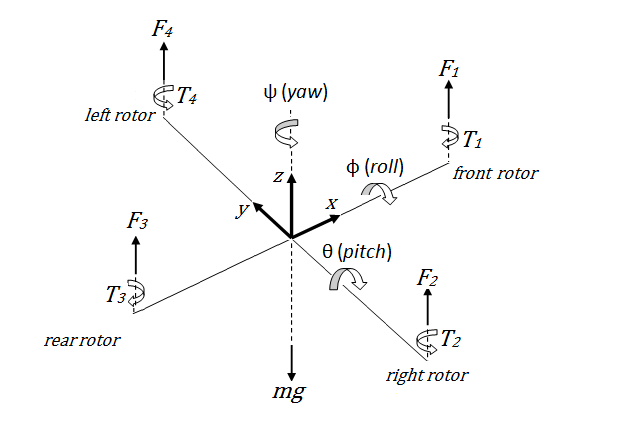
\includegraphics[width=.48\textwidth]{quadcopter}
\end{figure} 

\subsection{Governing Differential Equations of Motion}

\underline{\textbf{Inertial Frame Quantities:}}
$$\vect{P} = \bvecttrans{x}{y}{z} \quad \vect{V_{ref}} = \bvecttrans{\dot{x}}{\dot{y}}{\dot{z}}$$

\underline{\textbf{Body Frame Quantities:}}
$$ V_{body} = \bvecttrans{u}{v}{w} \quad , \omega^{body} = \bvecttrans{p}{q}{r}$$


$$\boxed{\bvectdot{u}{v}{w} = \frac{1}{m}\sum\vect{F} - \bvect{q w - r v}{r u -p w}{p v - q u}} $$

$$\boxed{ \bvectdot{p}{q}{r} = \bvect{\frac{\sum\tau_{1}}{I_{xx}}}{\frac{\sum\tau_{2}}{I_{yy}}}{\frac{\sum\tau_{3}}{I_{zz}}} - \bvect{\frac{(I_{zz} - I_{yy})}{I_{xx}}qr}{\frac{(I_{xx} - I_{zz})}{I_{yy}}pr}{\frac{(I_{yy}- I_{xx})}{I_{zz}}pq} \quad \quad \text{where} \quad \sum\vect{\tau} = \bvect{\sum\tau_{1}}{\sum\tau_{2}}{\sum\tau_{3}}}$$

$$\boxed{\sum F_{ext} \biggr\rvert_{body}= R_{zyx}(\phi, \theta, \psi)\biggr\rvert_{I}^{B}\left(\bvect{0}{0}{-mg} + \bvect{-k_d\dot{x}}{-k_d\dot{y}}{-k_d\dot{z}}\right) + k_{lift}\bvect{0}{0}{\sum\omega_{i}^{2}} }$$

$$\boxed{\tau_{body} = \bvect{\tau_{\phi}}{\tau_{\theta}}{\tau_{\psi}} = \bvect{Lk(\omega_{1}^{2} - \omega_{3}^{2})}{Lk(\omega_{2}^{2} - \omega_{4}^{2})}{b(\omega_{1}^{2}- \omega_{2}^{2} + \omega_{3}^{2} - \omega_{4}^{2})}}$$

$$ \bvect{p}{q}{r} = \begin{bmatrix}
    1 & 0 & -s(\theta)\\
    0 & c(\phi) & s(\phi)c(\theta)\\
    0 & -s(\phi) & c(\phi)c(\theta) \end{bmatrix}  \bvectdot{\phi}{\theta}{\psi}$$

$$ \bvectdot{\phi}{\theta}{\psi} = \begin{bmatrix}
    1 & s(\phi)t(\theta) & c(\phi)t(\theta)\\
    0 & c(\phi) & -s(\phi)\\
    0 & \frac{s(\phi)}{c(\theta)} & \frac{c(\phi)}{c(\theta)} \end{bmatrix} \bvect{p}{q}{r} $$

\section{Simulation}
Now that the dynamics of the system have been handled, we can turn to the simulation by preparing a State Space model of the quadcopter and then applying a feedback control system such that we can control the pose of the quadcopter in space and guide it to desirable positions. 

\subsection{State Space Formulation}

\subsubsection{System States \& Inputs}

While it is possible to further model the system by including the dynamics of the actuators (four electric motors), for simplicity this simulation will assume direct control to command exact motor speeds 
 
$$ \vect{U} = [\omega_1, \omega_2, \omega_3, \omega_4]^{T} $$
$$ \vect{Q} = \begin{bmatrix} 
u, v, w, p, q, r, \bar{q}, x, y, z
\end{bmatrix} $$

\subsubsection{Canonical State Space Form}

$$\dot{\vect{Q}} = \tilde{A}()\vect{Q} + \tilde{B}()\vect{U}$$
% $$\vect{Y} = \tilde{C}()\vect{Q} + \tilde{D}()\vect{U}$$


\subsubsection{Quadcopter State Space}

$$\bvectdot{x}{y}{z} = R(\bar{q})\bvect{u}{v}{w}$$

$$\bvectdot{u}{v}{w} = \frac{1}{m}\left(R(\bar{q})\biggr\rvert_{I}^{B}\left(\bvect{0}{0}{-mg} + \bvect{-k_d\dot{x}}{-k_d\dot{y}}{-k_d\dot{z}}\right) + k_{lift}\bvect{0}{0}{\sum\omega_{i}^{2}} \right) - \bvect{q w - r v}{r u -p w}{p v - q u}$$

$$\bvectdot{p}{q}{r} = \begin{bmatrix}
    \frac{1}{I_{xx}} & 0 & 0 \\
    0 & \frac{1}{I_{yy}} & 0 \\
    0 & 0 & \frac{1}{I_{zz}} \\
\end{bmatrix} \bvect{Lk(\omega_{1}^{2} - \omega_{3}^{2})}{Lk(\omega_{2}^{2} - \omega_{4}^{2})}{b(\omega_{1}^{2}- \omega_{2}^{2} + \omega_{3}^{2} - \omega_{4}^{2})}- \bvect{\frac{(I_{zz} - I_{yy})}{I_{xx}}qr}{\frac{(I_{xx} - I_{zz})}{I_{yy}}pr}{\frac{(I_{yy}- I_{xx})}{I_{zz}}pq}$$


% $$\begin{bmatrix}
%     \dot{u} \\
%     \dot{v} \\
%     \dot{w} \\
%     \dot{p} \\
%     \dot{q} \\
%     \dot{r} \\
%     \dot{x} \\
%     \dot{y} \\
%     \dot{z} \\
%     \dot{\bar{q}} \\
% \end{bmatrix} = A \begin{bmatrix}
%     u \\
%     v \\
%     w \\
%     p \\
%     q \\
%     r \\
%     x \\
%     y \\
%     z \\
%     \bar{q}
% \end{bmatrix} + B \begin{bmatrix}
%     U_1 \\
%     U_2 \\
%     U_3 \\
%     U_4 \\
% \end{bmatrix}$$

% $$$$

\subsection{Discretization Scheme}

\subsection{}



\printbibliography  

\end{document}